% !TEX encoding = UTF-8
% !TEX program = pdflatex
% !TEX root = AALP.tex
% !TEX spellcheck = it-IT

% 13 Ottobre 2016

% section semantica operazionale
%sub section call-by-name

\section{Sistemi di tipi}

\`E interessante studiare un sistema di tipi anche se molto semplice perché alla fine il pattern di ragionamento è lo stesso dei sistemi più complessi.

L'obiettivo di un sistema di tipi è che se si ha un programma $M$ ben tipato, allora $M$ non produce errore a run-time.

Perché il sistema funzioni è necessario avere:

\begin{itemize}
	\item Una \textbf{sintassi} che descrive il programma.
	\item Un controllo \textbf{statico} del sorgente del programma.
	\item Un ambiente \textbf{dinamico} per l'esecuzione (run-time) del programma. L'ambiente run-time è strettamente legato alla \textbf{semantica} del programma.
\end{itemize}

Considerando un insieme di programmi sintatticamente corretti, questo può essere diviso nell'insieme dei programma corretti semanticamente e quelli semanticamente errati. Tra quelli semanticamente \textbf{corretti} ci sono anche i programmi \textbf{ben tipati} che sono quei programmi che hanno anche i tipi corretti. Tipicamente il sotto-insieme dei programmi ben tipati non è completo, ovvero non contiene tutti i programmi semanticamente corretti. Questo però non è un problema.

Un errore semantico di un programma non è altro che un termine stuck, quindi quando un programma è ben tipato si ha la garanzia che l'esecuzione non finisca in un termine stuck.

Il tutto viene formalizzato dal \textbf{Teorema di safety}:

\begin{center}
	Se $M$ è ben tipato allora $M \not\rightarrow^* M'$ con $M'$ termine stuck\footnote{$\rightarrow^*$ indica la chiusura riflessiva transitiva di $\rightarrow$, ovvero indica una sequenza di passi.}
\end{center}

Per dimostrare la correttezza di questo teorema è necessario introdurre il \textbf{Teorema di Progressione}: se $M$ è ben tipato, allora $M$ non è stuck, cioè o $M$ è un valore, oppure $\exists M' \: M \rightarrow M'$.

Serve anche il \textbf{Teorema di Preservazione}: se $M$ è ben tipato e $M \rightarrow M'$ allora anche $M'$ è ben tipato.

Resta da formalizzare il concetto di ``\textit{ben tipato}''.
Se abbiamo un programma $M$ semanticamente corretto, sappiamo che data la nostra semantica deterministica o $M \rightarrow^* v$ oppure $M \rightarrow M' \text{stuck}$.
Si può quindi caratterizzare i possibili $v$ ed utilizzare il loro tipo per determinare il tipo del programma $M$.

Per esprimere il tipo di un termine viene utilizzata una \textbf{relazione di typing} $M : T$.
Nel nostro linguaggio funzionale i tipi possibili sono:

\begin{center}
$
T ::= \text{Bool} \:|\: \text{Nat} \:|\: T \rightarrow T
$ \footnote{Nat o Int, cambia poco}
\end{center}

Esempi di tipi:
\begin{itemize}
	\item $\fn x.\iif x \then 1 \eelse 0$ ha come tipo $\text{Bool} \rightarrow \text{Nat}$
	\item $\fn x.x$ ha più tipi possibili: $\text{Nat} \rightarrow \text{Nat}$, $\text{Bool} \rightarrow \text{Bool}$, ecc. Per gestire questa situazione richiediamo che venga esplicitamente espresso il tipo del parametro della funzione. Ottenendo quindi definizioni del tipo $\fn x : \text{Nat} .x$.
	\item $\fn y : \text{(Bool}\rightarrow\text{Nat) } . \fn z \text{: Bool }.\iff z \then 1 \eelse (y \: z)$ utilizza la notazione di tipo per i parametri delle due funzioni. Il tipo del programma risulta essere $\text{(Bool}\rightarrow \text{Nat)} \rightarrow \text{(Bool}\rightarrow \text{Nat)}$.
\end{itemize}

Può capitare che ci siano dei termini con delle variabili libere che devono essere tipate come $x + 1$.

In questo caso è necessario definire un \textbf{contesto}, ovvero una lista di tipi per le variabili.
Il contesto viene indicato formalmente con 

$$
\Gamma \vdash M : T
$$

Nell'esempio precedente si ha

$$
x : \text{ Nat } \vdash x + 1 : \text{ Nat}
$$

\subsection{Formalizzazione del sistema di tipi}

\begin{figure}[htbp]
	\centering
	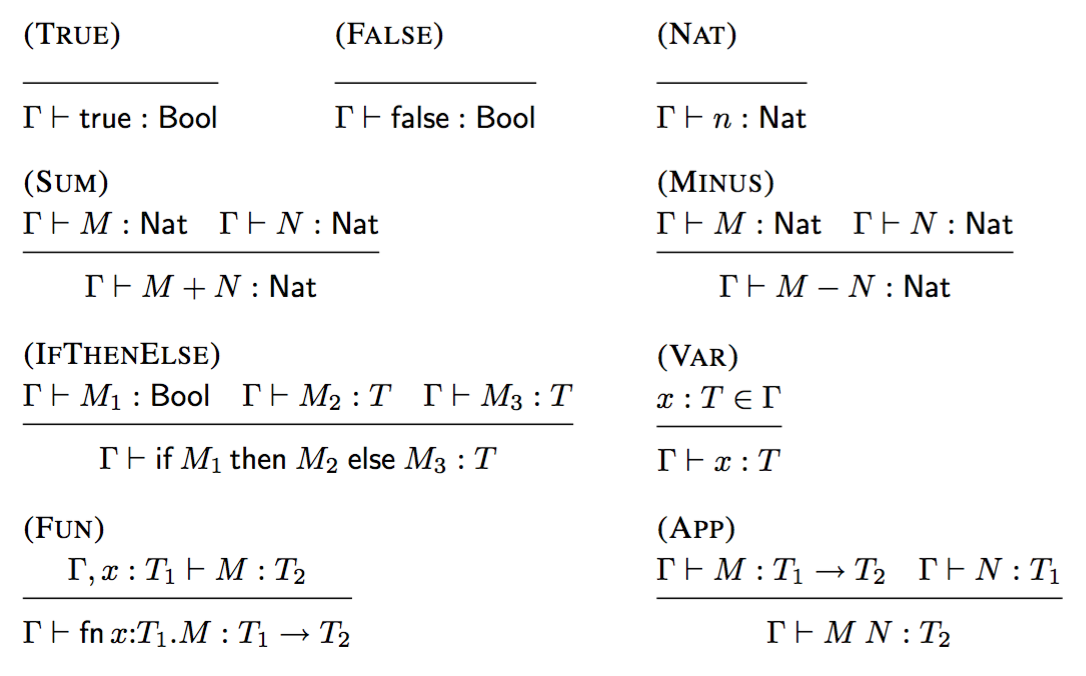
\includegraphics[width=0.6\textwidth]{images/l4-assiomi}
\end{figure}

Le ipotesi specificano che tipo devono avere i vari termini affinché valgano le regole e gli assiomi.

La regola \textsc{Fun} dice che il programma sarà ben tipato con il tipo $T_1 \rightarrow T_2$ se il corpo della funzione $M$ ha tipo $T_2$ assumendo il contesto $\Gamma$ e che $x : T_1$. Deve inoltre valere $x \not\in \Gamma$ per evitare conflitti di nomi, se questo non è vero basta effettuare una alpha-conversione sul parametro della funzione.

Alcuni esempi:

$$
	\emptyset \vdash \iif \true \then 5+7 \eelse 2 : \Nat
$$

\begin{prooftree}
	% Ramo 1
	\AxiomC{$\checkmark$}
	\LeftLabel{\textsc{(Bool)}}
	\UnaryInfC{$\emptyset \vdash \true : \Bool	$}
	% Ramo 2
	\AxiomC{$\checkmark$}
	\LeftLabel{\textsc{(Nat)}}
	\UnaryInfC{$\emptyset \vdash 5 : \Nat$}
	\AxiomC{$\checkmark$}
	\LeftLabel{\textsc{(Nat)}}
	\UnaryInfC{$\emptyset \vdash 7 : \Nat$}
	\LeftLabel{\textsc{(Sum)}}
	\BinaryInfC{$\emptyset \vdash 5+7 : \Nat $}
	% Ramo 3
	\AxiomC{$\checkmark$}
	\LeftLabel{\textsc{(Nat)}}
	\UnaryInfC{$\emptyset \vdash 2 : \Nat$}
	\LeftLabel{\textsc{(If)}}
	\TrinaryInfC{$\emptyset \vdash \iif \true \then 5+7 \eelse 2 : \Nat$}
\end{prooftree}

\vspace{30px}

$$
\emptyset \vdash \fn x : \Nat.\Big[ (\fn y : \Nat : \true) (x +1)\Big] : (\Nat \rightarrow \Bool)
$$

\begin{prooftree}
	%Ramo App-1
	\AxiomC{$\checkmark$}
	\LeftLabel{\textsc{(Bool)}}
	\UnaryInfC{$x:\Nat, y:\Nat \vdash \true : \Bool $}
	\LeftLabel{\textsc{(Fun)}}
	\UnaryInfC{$x : \Nat \vdash \fn y : \Nat . \true :\Bool $}
	
	%Ramo App-2
	% Ramo sum-1
	\AxiomC{$\checkmark$}
	\LeftLabel{\textsc{(Nat)}}
	\UnaryInfC{$x:\Nat \vdash x: \Nat$}
	% Ramo sum-2
	\AxiomC{$\checkmark$}
	\LeftLabel{\textsc{(Nat)}}
	\UnaryInfC{$x:\Nat \vdash 1: \Nat$}
	
	\LeftLabel{\textsc{(Sum)}}
	\BinaryInfC{$ x: \Nat \vdash x+1 : \Nat  $}
	\LeftLabel{\textsc{(App)}}
	\BinaryInfC{$x : \Nat \vdash (\fn y : \Nat . \true) (x +1) : \Bool$}
	\LeftLabel{\textsc{(Fun)}}
	\UnaryInfC{$\emptyset \vdash \fn x : \Nat.\Big[ (\fn y : \Nat . \true) (x +1)\Big] : (\Nat \rightarrow \Bool)$}
\end{prooftree}

\vspace{30px}

$$
\text{Definisci }\Gamma \text{ in modo che il programma sia ben tipato }\Gamma \vdash z (x y) : \Bool
$$\todo{todo}

\vspace{30px}

$$
\Gamma \vdash x \: x : T
$$\todo{todo}
